\documentclass{article}

\usepackage{graphicx}
\usepackage{amsmath}
\usepackage{amsthm}
\usepackage{amssymb}
\usepackage{fancyhdr}
\usepackage{hyperref}
\usepackage[dvipsnames]{xcolor}
\usepackage{enumitem}
\usepackage{minted}
\usepackage{listings}
\usepackage{minted}
%%%%% NEW MATH DEFINITIONS %%%%%

\usepackage{amsmath,amsfonts,bm,bbm}



\global\long\def\reals{\mathbb{R}}
 \global\long\def\integers{\mathbf{Z}}
\global\long\def\naturals{\mathbf{N}}
 \global\long\def\rationals{\mathbf{Q}}
\global\long\def\ca{\mathcal{A}}
\global\long\def\cb{\mathcal{B}}
 \global\long\def\cc{\mathcal{C}}
 \global\long\def\cd{\mathcal{D}}
\global\long\def\ce{\mathcal{E}}
\global\long\def\cf{\mathcal{F}}
\global\long\def\cg{\mathcal{G}}
\global\long\def\ch{\mathcal{H}}
\global\long\def\ci{\mathcal{I}}
\global\long\def\cj{\mathcal{J}}
\global\long\def\ck{\mathcal{K}}
\global\long\def\cl{\mathcal{L}}
\global\long\def\cm{\mathcal{M}}
\global\long\def\cn{\mathcal{N}}
\global\long\def\co{\mathcal{O}}
\global\long\def\cp{\mathcal{P}}
\global\long\def\cq{\mathcal{Q}}
\global\long\def\calr{\mathcal{R}}
\global\long\def\cs{\mathcal{S}}
\global\long\def\ct{\mathcal{T}}
\global\long\def\cu{\mathcal{U}}
\global\long\def\cv{\mathcal{V}}
\global\long\def\cw{\mathcal{W}}
\global\long\def\cx{\mathcal{X}}
\global\long\def\cy{\mathcal{Y}}
\global\long\def\cz{\mathcal{Z}}
\global\long\def\ind#1{1(#1)}
\global\long\def\pr{\mathbb{P}}

\global\long\def\ex{\mathbb{E}}
\global\long\def\var{\textrm{Var}}
\global\long\def\cov{\textrm{Cov}}
\global\long\def\sgn{\textrm{sgn}}
\global\long\def\sign{\textrm{sign}}
\global\long\def\kl{\textrm{KL}}
\global\long\def\law{\mathcal{L}}
\global\long\def\eps{\varepsilon}
\global\long\def\convd{\stackrel{d}{\to}}
\global\long\def\eqd{\stackrel{d}{=}}
\global\long\def\del{\nabla}
\global\long\def\loss{\ell}
\global\long\def\tr{\operatorname{tr}}
\global\long\def\trace{\operatorname{trace}}
\global\long\def\diag{\text{diag}}
\global\long\def\rank{\text{rank}}
\global\long\def\linspan{\text{span}}
\global\long\def\proj{\text{Proj}}
\global\long\def\argmax{\operatornamewithlimits{arg\, max}}
\global\long\def\argmin{\operatornamewithlimits{arg\, min}}
\global\long\def\bfx{\mathbf{x}}
\global\long\def\bfy{\mathbf{y}}
\global\long\def\bfl{\mathbf{\lambda}}
\global\long\def\bfm{\mathbf{\mu}}
\global\long\def\calL{\mathcal{L}}
\global\long\def\vw{\boldsymbol{w}}
\global\long\def\vx{\boldsymbol{x}}
\global\long\def\vxi{\boldsymbol{\xi}}
\global\long\def\valpha{\boldsymbol{\alpha}}
\global\long\def\vbeta{\boldsymbol{\beta}}
\global\long\def\vsigma{\boldsymbol{\sigma}}
\global\long\def\vmu{\boldsymbol{\mu}}
\global\long\def\vtheta{\boldsymbol{\theta}}
\global\long\def\vd{\boldsymbol{d}}
\global\long\def\vs{\boldsymbol{s}}
\global\long\def\vt{\boldsymbol{t}}
\global\long\def\vh{\boldsymbol{h}}
\global\long\def\ve{\boldsymbol{e}}
\global\long\def\vf{\boldsymbol{f}}
\global\long\def\vg{\boldsymbol{g}}
\global\long\def\vz{\boldsymbol{z}}
\global\long\def\vk{\boldsymbol{k}}
\global\long\def\va{\boldsymbol{a}}
\global\long\def\vb{\boldsymbol{b}}
\global\long\def\vv{\boldsymbol{v}}
\global\long\def\vy{\boldsymbol{y}}


%%%%%%%%%%%%%



\def\ind{{\mathbbm{1}}}

% Mark sections of captions for referring to divisions of figures
\newcommand{\figleft}{{\em (Left)}}
\newcommand{\figcenter}{{\em (Center)}}
\newcommand{\figright}{{\em (Right)}}
\newcommand{\figtop}{{\em (Top)}}
\newcommand{\figbottom}{{\em (Bottom)}}
\newcommand{\captiona}{{\em (a)}}
\newcommand{\captionb}{{\em (b)}}
\newcommand{\captionc}{{\em (c)}}
\newcommand{\captiond}{{\em (d)}}
\newcommand{\figleftt}{{\em Left}}
\newcommand{\figcentert}{{\em Center}}
\newcommand{\figrightt}{{\em Right}}
\newcommand{\figtopt}{{\em Top}}
\newcommand{\figbottomt}{{\em Bottom}}
\newcommand{\captionat}{{\em a}}
\newcommand{\captionbt}{{\em b}}
\newcommand{\captionct}{{\em c}}
\newcommand{\captiondt}{{\em d}}

% Highlight a newly defined term
\newcommand{\newterm}[1]{{\bf #1}}


% Figure reference, lower-case.
\def\figref#1{figure~\ref{#1}}
% Figure reference, capital. For start of sentence
\def\Figref#1{Figure~\ref{#1}}
\def\twofigref#1#2{figures \ref{#1} and \ref{#2}}
\def\quadfigref#1#2#3#4{figures \ref{#1}, \ref{#2}, \ref{#3} and \ref{#4}}
% Section reference, lower-case.
\def\secref#1{section~\ref{#1}}
% Section reference, capital.
\def\Secref#1{Section~\ref{#1}}
% Reference to two sections.
\def\twosecrefs#1#2{sections \ref{#1} and \ref{#2}}
% Reference to three sections.
\def\secrefs#1#2#3{sections \ref{#1}, \ref{#2} and \ref{#3}}

\def\chapref#1{chapter~\ref{#1}}
% Reference to an equation, upper case.
\def\Chapref#1{Chapter~\ref{#1}}
% Reference to a range of chapters
\def\rangechapref#1#2{chapters\ref{#1}--\ref{#2}}
% Reference to an algorithm, lower-case.
\def\algref#1{algorithm~\ref{#1}}
% Reference to an algorithm, upper case.
\def\Algref#1{Algorithm~\ref{#1}}
\def\twoalgref#1#2{algorithms \ref{#1} and \ref{#2}}
\def\Twoalgref#1#2{Algorithms \ref{#1} and \ref{#2}}
% Reference to a part, lower case
\def\partref#1{part~\ref{#1}}
% Reference to a part, upper case
\def\Partref#1{Part~\ref{#1}}
\def\twopartref#1#2{parts \ref{#1} and \ref{#2}}

\def\ceil#1{\lceil #1 \rceil}
\def\floor#1{\lfloor #1 \rfloor}
\def\1{\bm{1}}
\newcommand{\train}{\mathcal{D}}
\newcommand{\valid}{\mathcal{D_{\mathrm{valid}}}}
\newcommand{\test}{\mathcal{D_{\mathrm{test}}}}

\def\eps{{\epsilon}}


% Random variables
\def\reta{{\textnormal{$\eta$}}}
\def\ra{{\textnormal{a}}}
\def\rb{{\textnormal{b}}}
\def\rc{{\textnormal{c}}}
\def\rd{{\textnormal{d}}}
\def\re{{\textnormal{e}}}
\def\rf{{\textnormal{f}}}
\def\rg{{\textnormal{g}}}
\def\rh{{\textnormal{h}}}
\def\ri{{\textnormal{i}}}
\def\rj{{\textnormal{j}}}
\def\rk{{\textnormal{k}}}
\def\rl{{\textnormal{l}}}
% rm is already a command, just don't name any random variables m
\def\rn{{\textnormal{n}}}
\def\ro{{\textnormal{o}}}
\def\rp{{\textnormal{p}}}
\def\rq{{\textnormal{q}}}
\def\rr{{\textnormal{r}}}
\def\rs{{\textnormal{s}}}
\def\rt{{\textnormal{t}}}
\def\ru{{\textnormal{u}}}
\def\rv{{\textnormal{v}}}
\def\rw{{\textnormal{w}}}
\def\rx{{\textnormal{x}}}
\def\ry{{\textnormal{y}}}
\def\rz{{\textnormal{z}}}

% Random vectors
\def\rvepsilon{{\mathbf{\epsilon}}}
\def\rvtheta{{\mathbf{\theta}}}
\def\rva{{\mathbf{a}}}
\def\rvb{{\mathbf{b}}}
\def\rvc{{\mathbf{c}}}
\def\rvd{{\mathbf{d}}}
\def\rve{{\mathbf{e}}}
\def\rvf{{\mathbf{f}}}
\def\rvg{{\mathbf{g}}}
\def\rvh{{\mathbf{h}}}
\def\rvu{{\mathbf{i}}}
\def\rvj{{\mathbf{j}}}
\def\rvk{{\mathbf{k}}}
\def\rvl{{\mathbf{l}}}
\def\rvm{{\mathbf{m}}}
\def\rvn{{\mathbf{n}}}
\def\rvo{{\mathbf{o}}}
\def\rvp{{\mathbf{p}}}
\def\rvq{{\mathbf{q}}}
\def\rvr{{\mathbf{r}}}
\def\rvs{{\mathbf{s}}}
\def\rvt{{\mathbf{t}}}
\def\rvu{{\mathbf{u}}}
\def\rvv{{\mathbf{v}}}
\def\rvw{{\mathbf{w}}}
\def\rvx{{\mathbf{x}}}
\def\rvy{{\mathbf{y}}}
\def\rvz{{\mathbf{z}}}

% Elements of random vectors
\def\erva{{\textnormal{a}}}
\def\ervb{{\textnormal{b}}}
\def\ervc{{\textnormal{c}}}
\def\ervd{{\textnormal{d}}}
\def\erve{{\textnormal{e}}}
\def\ervf{{\textnormal{f}}}
\def\ervg{{\textnormal{g}}}
\def\ervh{{\textnormal{h}}}
\def\ervi{{\textnormal{i}}}
\def\ervj{{\textnormal{j}}}
\def\ervk{{\textnormal{k}}}
\def\ervl{{\textnormal{l}}}
\def\ervm{{\textnormal{m}}}
\def\ervn{{\textnormal{n}}}
\def\ervo{{\textnormal{o}}}
\def\ervp{{\textnormal{p}}}
\def\ervq{{\textnormal{q}}}
\def\ervr{{\textnormal{r}}}
\def\ervs{{\textnormal{s}}}
\def\ervt{{\textnormal{t}}}
\def\ervu{{\textnormal{u}}}
\def\ervv{{\textnormal{v}}}
\def\ervw{{\textnormal{w}}}
\def\ervx{{\textnormal{x}}}
\def\ervy{{\textnormal{y}}}
\def\ervz{{\textnormal{z}}}

% Random matrices
\def\rmA{{\mathbf{A}}}
\def\rmB{{\mathbf{B}}}
\def\rmC{{\mathbf{C}}}
\def\rmD{{\mathbf{D}}}
\def\rmE{{\mathbf{E}}}
\def\rmF{{\mathbf{F}}}
\def\rmG{{\mathbf{G}}}
\def\rmH{{\mathbf{H}}}
\def\rmI{{\mathbf{I}}}
\def\rmJ{{\mathbf{J}}}
\def\rmK{{\mathbf{K}}}
\def\rmL{{\mathbf{L}}}
\def\rmM{{\mathbf{M}}}
\def\rmN{{\mathbf{N}}}
\def\rmO{{\mathbf{O}}}
\def\rmP{{\mathbf{P}}}
\def\rmQ{{\mathbf{Q}}}
\def\rmR{{\mathbf{R}}}
\def\rmS{{\mathbf{S}}}
\def\rmT{{\mathbf{T}}}
\def\rmU{{\mathbf{U}}}
\def\rmV{{\mathbf{V}}}
\def\rmW{{\mathbf{W}}}
\def\rmX{{\mathbf{X}}}
\def\rmY{{\mathbf{Y}}}
\def\rmZ{{\mathbf{Z}}}
\def\rmtheta{{\mathbf{\Theta}}}
% Elements of random matrices
\def\ermA{{\textnormal{A}}}
\def\ermB{{\textnormal{B}}}
\def\ermC{{\textnormal{C}}}
\def\ermD{{\textnormal{D}}}
\def\ermE{{\textnormal{E}}}
\def\ermF{{\textnormal{F}}}
\def\ermG{{\textnormal{G}}}
\def\ermH{{\textnormal{H}}}
\def\ermI{{\textnormal{I}}}
\def\ermJ{{\textnormal{J}}}
\def\ermK{{\textnormal{K}}}
\def\ermL{{\textnormal{L}}}
\def\ermM{{\textnormal{M}}}
\def\ermN{{\textnormal{N}}}
\def\ermO{{\textnormal{O}}}
\def\ermP{{\textnormal{P}}}
\def\ermQ{{\textnormal{Q}}}
\def\ermR{{\textnormal{R}}}
\def\ermS{{\textnormal{S}}}
\def\ermT{{\textnormal{T}}}
\def\ermU{{\textnormal{U}}}
\def\ermV{{\textnormal{V}}}
\def\ermW{{\textnormal{W}}}
\def\ermX{{\textnormal{X}}}
\def\ermY{{\textnormal{Y}}}
\def\ermZ{{\textnormal{Z}}}

% Vectors
\def\vzero{{\bm{0}}}
\def\vone{{\bm{1}}}
\def\vmu{{\bm{\mu}}}
\def\vtheta{{\bm{\theta}}}
\def\va{{\bm{a}}}
\def\vb{{\bm{b}}}
\def\vc{{\bm{c}}}
\def\vd{{\bm{d}}}
\def\ve{{\bm{e}}}
\def\vf{{\bm{f}}}
\def\vg{{\bm{g}}}
\def\vh{{\bm{h}}}
\def\vi{{\bm{i}}}
\def\vj{{\bm{j}}}
\def\vk{{\bm{k}}}
\def\vl{{\bm{l}}}
\def\vm{{\bm{m}}}
\def\vn{{\bm{n}}}
\def\vo{{\bm{o}}}
\def\vp{{\bm{p}}}
\def\vq{{\bm{q}}}
\def\vr{{\bm{r}}}
\def\vs{{\bm{s}}}
\def\vt{{\bm{t}}}
\def\vu{{\bm{u}}}
\def\vv{{\bm{v}}}
\def\vw{{\bm{w}}}
\def\vx{{\bm{x}}}
\def\vy{{\bm{y}}}
\def\vz{{\bm{z}}}

% Elements of vectors
\def\evalpha{{\alpha}}
\def\evbeta{{\beta}}
\def\evepsilon{{\epsilon}}
\def\evlambda{{\lambda}}
\def\evomega{{\omega}}
\def\evmu{{\mu}}
\def\evpsi{{\psi}}
\def\evsigma{{\sigma}}
\def\evtheta{{\theta}}
\def\eva{{a}}
\def\evb{{b}}
\def\evc{{c}}
\def\evd{{d}}
\def\eve{{e}}
\def\evf{{f}}
\def\evg{{g}}
\def\evh{{h}}
\def\evi{{i}}
\def\evj{{j}}
\def\evk{{k}}
\def\evl{{l}}
\def\evm{{m}}
\def\evn{{n}}
\def\evo{{o}}
\def\evp{{p}}
\def\evq{{q}}
\def\evr{{r}}
\def\evs{{s}}
\def\evt{{t}}
\def\evu{{u}}
\def\evv{{v}}
\def\evw{{w}}
\def\evx{{x}}
\def\evy{{y}}
\def\evz{{z}}

% Matrix
\def\mA{{\bm{A}}}
\def\mB{{\bm{B}}}
\def\mC{{\bm{C}}}
\def\mD{{\bm{D}}}
\def\mE{{\bm{E}}}
\def\mF{{\bm{F}}}
\def\mG{{\bm{G}}}
\def\mH{{\bm{H}}}
\def\mI{{\bm{I}}}
\def\mJ{{\bm{J}}}
\def\mK{{\bm{K}}}
\def\mL{{\bm{L}}}
\def\mM{{\bm{M}}}
\def\mN{{\bm{N}}}
\def\mO{{\bm{O}}}
\def\mP{{\bm{P}}}
\def\mQ{{\bm{Q}}}
\def\mR{{\bm{R}}}
\def\mS{{\bm{S}}}
\def\mT{{\bm{T}}}
\def\mU{{\bm{U}}}
\def\mV{{\bm{V}}}
\def\mW{{\bm{W}}}
\def\mX{{\bm{X}}}
\def\mY{{\bm{Y}}}
\def\mZ{{\bm{Z}}}
\def\mBeta{{\bm{\beta}}}
\def\mPhi{{\bm{\Phi}}}
\def\mLambda{{\bm{\Lambda}}}
\def\mSigma{{\bm{\Sigma}}}

% Tensor
\DeclareMathAlphabet{\mathsfit}{\encodingdefault}{\sfdefault}{m}{sl}
\SetMathAlphabet{\mathsfit}{bold}{\encodingdefault}{\sfdefault}{bx}{n}
\newcommand{\tens}[1]{\bm{\mathsfit{#1}}}
\def\tA{{\tens{A}}}
\def\tB{{\tens{B}}}
\def\tC{{\tens{C}}}
\def\tD{{\tens{D}}}
\def\tE{{\tens{E}}}
\def\tF{{\tens{F}}}
\def\tG{{\tens{G}}}
\def\tH{{\tens{H}}}
\def\tI{{\tens{I}}}
\def\tJ{{\tens{J}}}
\def\tK{{\tens{K}}}
\def\tL{{\tens{L}}}
\def\tM{{\tens{M}}}
\def\tN{{\tens{N}}}
\def\tO{{\tens{O}}}
\def\tP{{\tens{P}}}
\def\tQ{{\tens{Q}}}
\def\tR{{\tens{R}}}
\def\tS{{\tens{S}}}
\def\tT{{\tens{T}}}
\def\tU{{\tens{U}}}
\def\tV{{\tens{V}}}
\def\tW{{\tens{W}}}
\def\tX{{\tens{X}}}
\def\tY{{\tens{Y}}}
\def\tZ{{\tens{Z}}}


% Graph
\def\gA{{\mathcal{A}}}
\def\gB{{\mathcal{B}}}
\def\gC{{\mathcal{C}}}
\def\gD{{\mathcal{D}}}
\def\gE{{\mathcal{E}}}
\def\gF{{\mathcal{F}}}
\def\gG{{\mathcal{G}}}
\def\gH{{\mathcal{H}}}
\def\gI{{\mathcal{I}}}
\def\gJ{{\mathcal{J}}}
\def\gK{{\mathcal{K}}}
\def\gL{{\mathcal{L}}}
\def\gM{{\mathcal{M}}}
\def\gN{{\mathcal{N}}}
\def\gO{{\mathcal{O}}}
\def\gP{{\mathcal{P}}}
\def\gQ{{\mathcal{Q}}}
\def\gR{{\mathcal{R}}}
\def\gS{{\mathcal{S}}}
\def\gT{{\mathcal{T}}}
\def\gU{{\mathcal{U}}}
\def\gV{{\mathcal{V}}}
\def\gW{{\mathcal{W}}}
\def\gX{{\mathcal{X}}}
\def\gY{{\mathcal{Y}}}
\def\gZ{{\mathcal{Z}}}

% Sets
\def\sA{{\mathbb{A}}}
\def\sB{{\mathbb{B}}}
\def\sC{{\mathbb{C}}}
\def\sD{{\mathbb{D}}}
% Don't use a set called E, because this would be the same as our symbol
% for expectation.
\def\sF{{\mathbb{F}}}
\def\sG{{\mathbb{G}}}
\def\sH{{\mathbb{H}}}
\def\sI{{\mathbb{I}}}
\def\sJ{{\mathbb{J}}}
\def\sK{{\mathbb{K}}}
\def\sL{{\mathbb{L}}}
\def\sM{{\mathbb{M}}}
\def\sN{{\mathbb{N}}}
\def\sO{{\mathbb{O}}}
\def\sP{{\mathbb{P}}}
\def\sQ{{\mathbb{Q}}}
\def\sR{{\mathbb{R}}}
\def\sS{{\mathbb{S}}}
\def\sT{{\mathbb{T}}}
\def\sU{{\mathbb{U}}}
\def\sV{{\mathbb{V}}}
\def\sW{{\mathbb{W}}}
\def\sX{{\mathbb{X}}}
\def\sY{{\mathbb{Y}}}
\def\sZ{{\mathbb{Z}}}

% Entries of a matrix
\def\emLambda{{\Lambda}}
\def\emA{{A}}
\def\emB{{B}}
\def\emC{{C}}
\def\emD{{D}}
\def\emE{{E}}
\def\emF{{F}}
\def\emG{{G}}
\def\emH{{H}}
\def\emI{{I}}
\def\emJ{{J}}
\def\emK{{K}}
\def\emL{{L}}
\def\emM{{M}}
\def\emN{{N}}
\def\emO{{O}}
\def\emP{{P}}
\def\emQ{{Q}}
\def\emR{{R}}
\def\emS{{S}}
\def\emT{{T}}
\def\emU{{U}}
\def\emV{{V}}
\def\emW{{W}}
\def\emX{{X}}
\def\emY{{Y}}
\def\emZ{{Z}}
\def\emSigma{{\Sigma}}

% entries of a tensor
% Same font as tensor, without \bm wrapper
\newcommand{\etens}[1]{\mathsfit{#1}}
\def\etLambda{{\etens{\Lambda}}}
\def\etA{{\etens{A}}}
\def\etB{{\etens{B}}}
\def\etC{{\etens{C}}}
\def\etD{{\etens{D}}}
\def\etE{{\etens{E}}}
\def\etF{{\etens{F}}}
\def\etG{{\etens{G}}}
\def\etH{{\etens{H}}}
\def\etI{{\etens{I}}}
\def\etJ{{\etens{J}}}
\def\etK{{\etens{K}}}
\def\etL{{\etens{L}}}
\def\etM{{\etens{M}}}
\def\etN{{\etens{N}}}
\def\etO{{\etens{O}}}
\def\etP{{\etens{P}}}
\def\etQ{{\etens{Q}}}
\def\etR{{\etens{R}}}
\def\etS{{\etens{S}}}
\def\etT{{\etens{T}}}
\def\etU{{\etens{U}}}
\def\etV{{\etens{V}}}
\def\etW{{\etens{W}}}
\def\etX{{\etens{X}}}
\def\etY{{\etens{Y}}}
\def\etZ{{\etens{Z}}}


\DeclareMathOperator{\E}{\mathbb{E}}
\newcommand{\Ls}{\mathcal{L}}
\newcommand{\R}{\mathbb{R}}
\newcommand{\emp}{\tilde{p}}
\newcommand{\lr}{\alpha}
\newcommand{\reg}{\lambda}
\newcommand{\sigmoid}{\sigma}
\newcommand{\softplus}{\zeta}
\newcommand{\KL}{D_{\mathrm{KL}}}
\newcommand{\Var}{\mathrm{Var}}
\newcommand{\standarderror}{\mathrm{SE}}
\newcommand{\Cov}{\mathrm{Cov}}
% \DeclareMathOperator*{\argmax}{arg\,max}
% \DeclareMathOperator*{\argmin}{arg\,min}

% \DeclareMathOperator{\sign}{sign}
\DeclareMathOperator{\Tr}{Tr}
\let\ab\allowbreak

\newcommand{\vbar}[1]{\bigg\rvert_{#1}}
\newcommand\at[2]{\left.#1\right|_{#2}}
\newcommand{\bs}[1]{\boldsymbol{#1}}

\newcommand{\sigx}[1]{\sigma_{x,#1}}
\newcommand{\sigb}[1]{\sigma_{\beta,#1}}

\newcommand{\dd}{\mathrm{d}} %for integration

\newcommand{\wipcom}[1]{\textcolor{red}{WIP: #1}}
\newcommand{\sol}[1]{\textcolor{gray}{sol: #1}}
% \newcommand{\sol}[1]{}
\newcommand{\nyuparagraph}[1]{\vspace{0.3cm}\textcolor{nyupurple}{\bf \large #1}\\}
\newcommand{\code}[1]{\texttt{#1}}
\newcommand{\nll}{\rm NLL}


\pagestyle{empty} \addtolength{\textwidth}{1.0in}
\addtolength{\textheight}{0.5in} \addtolength{\oddsidemargin}{-0.5in}
\addtolength{\evensidemargin}{0.5in}
\newcommand{\ruleskip}{\bigskip\hrule\bigskip}
\newcommand{\nodify}[1]{{\sc #1}} \newcommand{\points}[1]{{\textbf{[#1
points]}}}

\newcommand{\bitem}{\begin{list}{$\bullet$}%
{\setlength{\itemsep}{0pt}\setlength{\topsep}{0pt}%
\setlength{\rightmargin}{0pt}}} \newcommand{\eitem}{\end{list}}

\definecolor{nyupurple}{RGB}{134, 0, 179}
\setlength{\parindent}{0pt} \setlength{\parskip}{0.5ex}

\DeclareUnicodeCharacter{2212}{-}

\theoremstyle{plain}
\newtheorem*{thm*}{\protect\theoremname}
\theoremstyle{definition}
\newtheorem*{defn*}{\protect\definitionname}

\begin{document}
\newcounter{saveenum}

\pagestyle{myheadings} \markboth{}{\color{nyupurple} DS-GA-1003 - Spring 2022}

\begin{center}
{\Large
Homework 7: Computation Graphs, Back-propagation, and Neural Networks
} 
\end{center}

{
{ \color{nyupurple} \textbf{Due:} Friday, May 6th, 2022 at 11:59PM EST} 
} 

\textbf{Instructions: }Your answers to the questions below, including plots and mathematical work, should be submitted as a single PDF file.  It's preferred that you write your answers using software that typesets mathematics (e.g.LaTeX, LyX, or MathJax via iPython), though if you need to you may scan handwritten work.  You may find the \href{https://github.com/gpoore/minted}{minted} package convenient for including source code in your LaTeX document.  If you are using LyX, then the \href{https://en.wikibooks.org/wiki/LaTeX/Source_Code_Listings}{listings} package tends to work better. 

\ruleskip

\section{Introduction}

There is no doubt that neural networks are a very important class
of machine learning models. Given the sheer number of people who are
achieving impressive results with neural networks, one might think
that it's relatively easy to get them working. This is a partly an
illusion. One reason so many people have success is that, thanks to
GitHub, they can copy the exact settings that others have used to
achieve success. In fact, in most cases they can start with ``pre-trained''
models that already work for a similar problem, and ``fine-tune''
them for their own purposes. It's far easier to tweak and improve
a working system than to get one working from scratch. If you create
a new model, you're kind of on your own to figure out how to get it
working: there's not much theory to guide you and the rules of thumb
do not always work. Understanding even the most basic questions, such
as the preferred variant of SGD to use for optimization, is still
a very active area of research.

One thing is clear, however: If you do need to start from scratch,
or debug a neural network model that doesn't seem to be learning,
it can be immensely helpful to understand the low-level details of
how your neural network works -- specifically, back-propagation.
With this assignment, you'll have the opportunity to linger on these
low-level implementation details. Every major neural network type
(RNNs, CNNs, Resnets, etc.) can be implemented using the basic framework
we'll develop in this assignment.

To help things along, Philipp Meerkamp, Pierre Garapon, and David Rosenberg
have designed a minimalist framework for computation graphs and put
together some support code. The intent is for you to read, or at least
skim, every line of code provided, so that you'll know you understand
all the crucial components and could, in theory, create your own from
scratch. In fact, creating your own computation graph framework from
scratch is highly encouraged -- you'll learn a lot. 

\section{Computation Graph Framework }

To get started, please read the \href{https://github.com/davidrosenberg/mlcourse/blob/gh-pages/Notebooks/computation-graph/computation-graph-framework.ipynb}{tutorial}
on the computation graph framework we'll be working with. (Note that
it renders better if you view it locally.) The use of computation
graphs is not specific to machine learning or neural networks. Computation
graphs are just a way to represent a function that facilitates efficient
computation of the function's values and its gradients with respect
to inputs. The tutorial takes this perspective, and there is very
little in it about machine learning, per se. 

To see how the framework can be used for machine learning tasks, we've
provided a full implementation of linear regression. You should start
by working your way through the \texttt{\_\_init\_\_} of the \texttt{LinearRegression}
class in \texttt{linear\_regression.py}. From there, you'll want to
review the node class definitions in \texttt{nodes.py}, and finally
the class \texttt{ComputationGraphFunction} in \texttt{graph.py}. \texttt{ComputationGraphFunction}
is where we repackage a raw computation graph into something that's
more friendly to work with for machine learning. The rest of \texttt{linear\_regression.py}
is fairly routine, but it illustrates how to interact with the \texttt{ComputationGraphFunction}.

As we've noted earlier in the course, getting gradient calculations
correct can be difficult. To help things along, we've provided two
functions that can be used to test the backward method of a node and
the overall gradient calculation of a \texttt{ComputationGraphFunction}.
The functions are in \texttt{test\_utils.py}, and it's recommended
that you review the tests provided for the linear regression implementation
in \texttt{linear\_regression.t.py}. (You can run these tests from
the command line with \texttt{python3 linear\_regression.t.py.}) The
functions actually doing the testing, \texttt{test\_node\_backward}
and \texttt{test\_ComputationGraphFunction}, may seem a bit intricate,
but they're implementing the exact same \texttt{gradient\_checker}
logic we saw in the second homework assignment.

Once you've understood how linear regression works in our framework,
you're ready to start implementing your own algorithms. To help you get started, please make sure you are able to execute the following commands:
\begin{itemize}
    \item cd /path/to/hw7
    \item python3 linear\_regression.py
    \item python3 linear\_regression.t.py
\end{itemize}

\section{Ridge Regression}

When moving to a new system, it's always good to start with something
familiar. But that's not the only reason we're doing ridge regression
in this homework. In ridge regression the
parameter vector is ``shared'', in the sense that it's used twice
in the objective function. In the computation graph, this can be seen
in the fact that the node for the parameter vector has two outgoing
edges. 
This sharing is common many popular neural networks (RNNs and CNNs), where it is often referred to as \emph{parameter tying}.

\texttt{ridge\_regression.py} provides a skeleton code
and \texttt{ridge\_regression.t.py} is a test code, which you should
eventually be able to pass.
\begin{enumerate}
\setcounter{enumi}{\value{saveenum}}

\newpage 

\item Complete the class \texttt{L2NormPenaltyNode} in \texttt{nodes.py}. If your code is correct, you should be able to pass test\_L2NormPenaltyNode in \texttt{ridge\_regression.t.py}. Please attach a screenshot that shows the test results for this question.

\begin{figure}[h!]
    \centering
    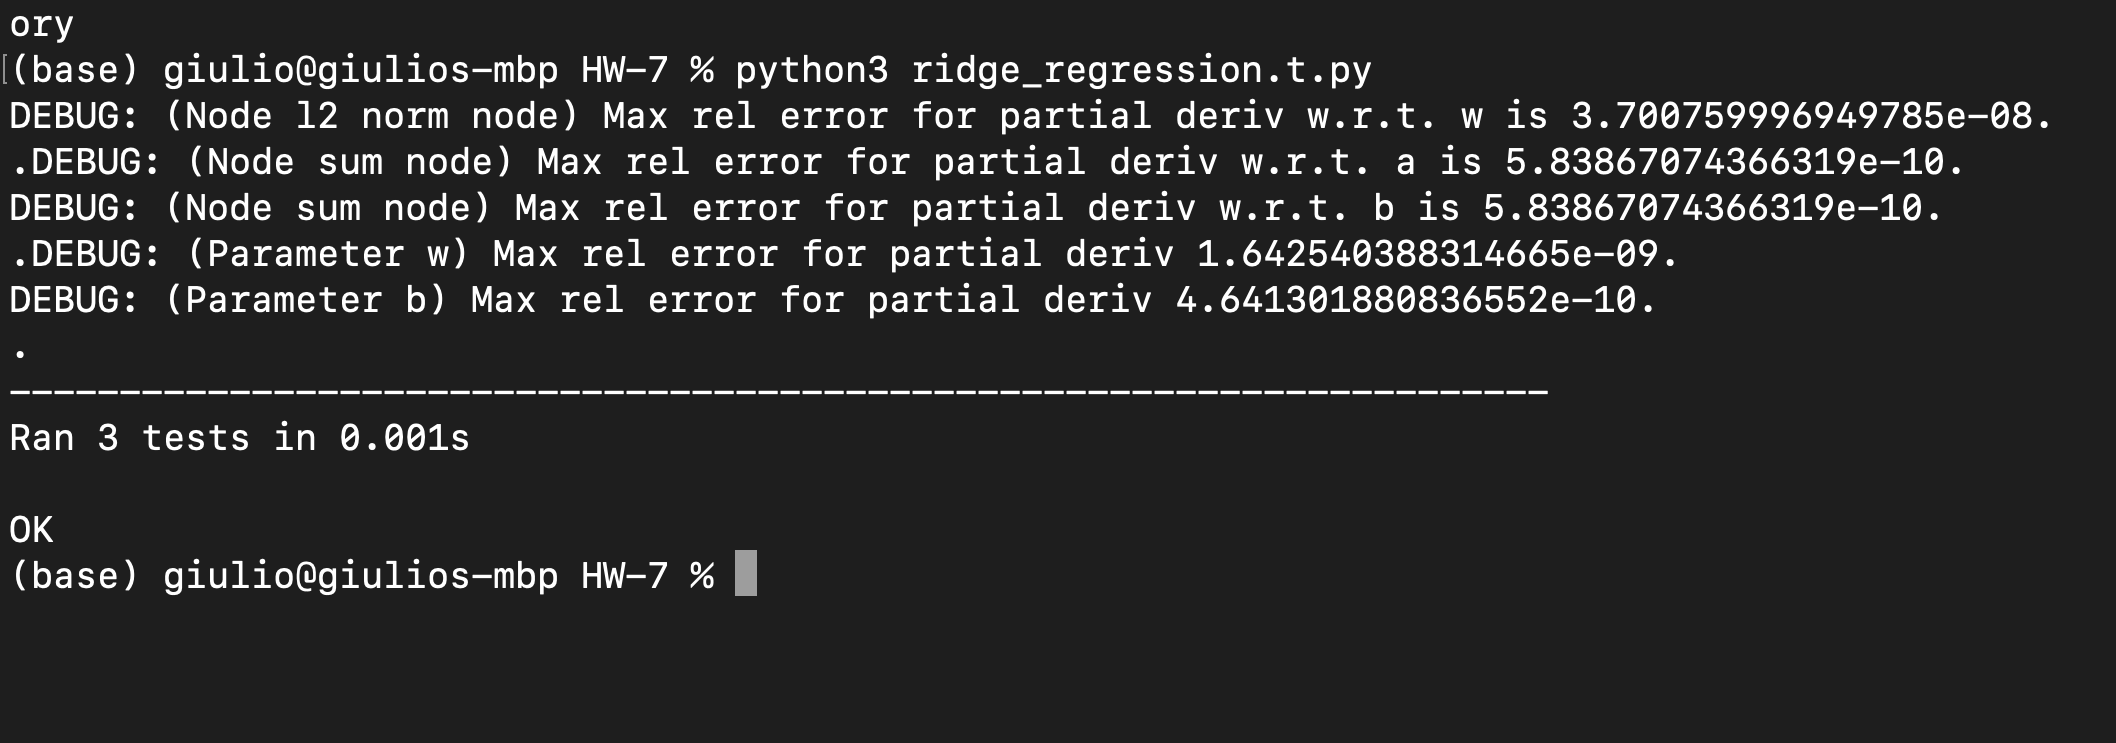
\includegraphics[scale=.4]{Ridge Regression Test Outputs.png}
    \caption{Ridge Regression Test Output}
    \label{fig:Ridge test}
\end{figure}
\subitem

\begin{minted}{Python}
class L2NormPenaltyNode(object):
    """ Node computing l2_reg * ||w||^2 for scalars l2_reg and vector w"""
    def __init__(self, l2_reg, w, node_name):
        """ 
        Parameters:
        l2_reg: a numpy scalar array (e.g. np.array(.01)) (not a node)
        w: a node for which w.out is a numpy vector
        node_name: node's name (a string)
        """
        self.node_name = node_name
        self.out = None
        self.d_out = None
        self.l2_reg = np.array(l2_reg)
        self.w = w

    def forward(self):
        self.out = self.l2_reg * np.dot(self.w.out,self.w.out)
        self.d_out = np.zeros(self.out.shape)
        return self.out

    def backward(self):
        d_w = 2 * self.w.out * self.l2_reg * self.d_out
        self.w.d_out += d_w
        return self.d_out
        
    def get_predecessors(self):
        ## Your code
        return [self.w]
\end{minted}

\item Complete the class \texttt{SumNode} in \texttt{nodes.py}. If your code is correct, you should be able to pass test\_SumNode in \texttt{ridge\_regression.t.py}. Please attach a screenshot that shows the test results for this question. 

\subitem

\begin{minted}{Python}
class SumNode(object):
    """ Node computing a + b, for numpy arrays a and b"""
    def __init__(self, a, b, node_name):
        """ 
        Parameters:
        a: node for which a.out is a numpy array
        b: node for which b.out is a numpy array of the same shape as a
        node_name: node's name (a string)
        """
        self.node_name = node_name
        self.out = None
        self.d_out = None
        self.b = b
        self.a = a

    def forward(self):
        self.out = self.a.out + self.b.out
        self.d_out = np.zeros(self.out.shape)
        return self.out

    def backward(self):
        #Derivative of a+b with respect to either is just 1
        self.a.d_out += self.d_out
        self.b.d_out += self.d_out
        return self.d_out

    def get_predecessors(self):
        # Your code
        return [self.a,self.b]
\end{minted}

\item Implement ridge regression with $w$ regularized and $b$ unregularized. Do this by completing the \texttt{\_\_init\_\_} method in \texttt{ridge\_regression.py},
using the classes created above. When complete, you should be able
to pass the tests in \texttt{ridge\_regression.t.py}. Report the average
square error on the \textbf{training} set for the parameter settings
given in the \texttt{main()} function. 

\subitem
\newpage

\begin{minted}{Python}
class RidgeRegression(BaseEstimator, RegressorMixin):
    """ Ridge regression with computation graph """
    def __init__(self, l2_reg=1, step_size=.005,  max_num_epochs = 5000):
        self.max_num_epochs = max_num_epochs
        self.step_size = step_size

        # Build computation graph
        self.x = nodes.ValueNode(node_name="x") # to hold a vector input
        self.y = nodes.ValueNode(node_name="y") # to hold a scalar response
        self.w = nodes.ValueNode(node_name="w") # to hold the parameter vector
        self.b = nodes.ValueNode(node_name="b") # to hold the bias parameter (scalar)
        self.prediction = nodes.VectorScalarAffineNode(x=self.x, w=self.w, b=self.b,
                                                 node_name="prediction")

        self.objective = nodes.SquaredL2DistanceNode(a=self.prediction, b=self.y,
                                               node_name="square loss")
        self.reg_loss = nodes.L2NormPenaltyNode(l2_reg=l2_reg, w=self.w,node_name = "reg_loss")
        self.loss = nodes.SumNode(a = self.objective,b = self.reg_loss, node_name="loss")
        
        self.inputs = [self.x]
        self.outcomes = [self.y]
        self.parameters = [self.w, self.b]

        self.graph = graph.ComputationGraphFunction(self.inputs, self.outcomes,
                                                          self.parameters, self.prediction,
                                                          self.loss)
\end{minted}

\begin{figure}
    \centering
    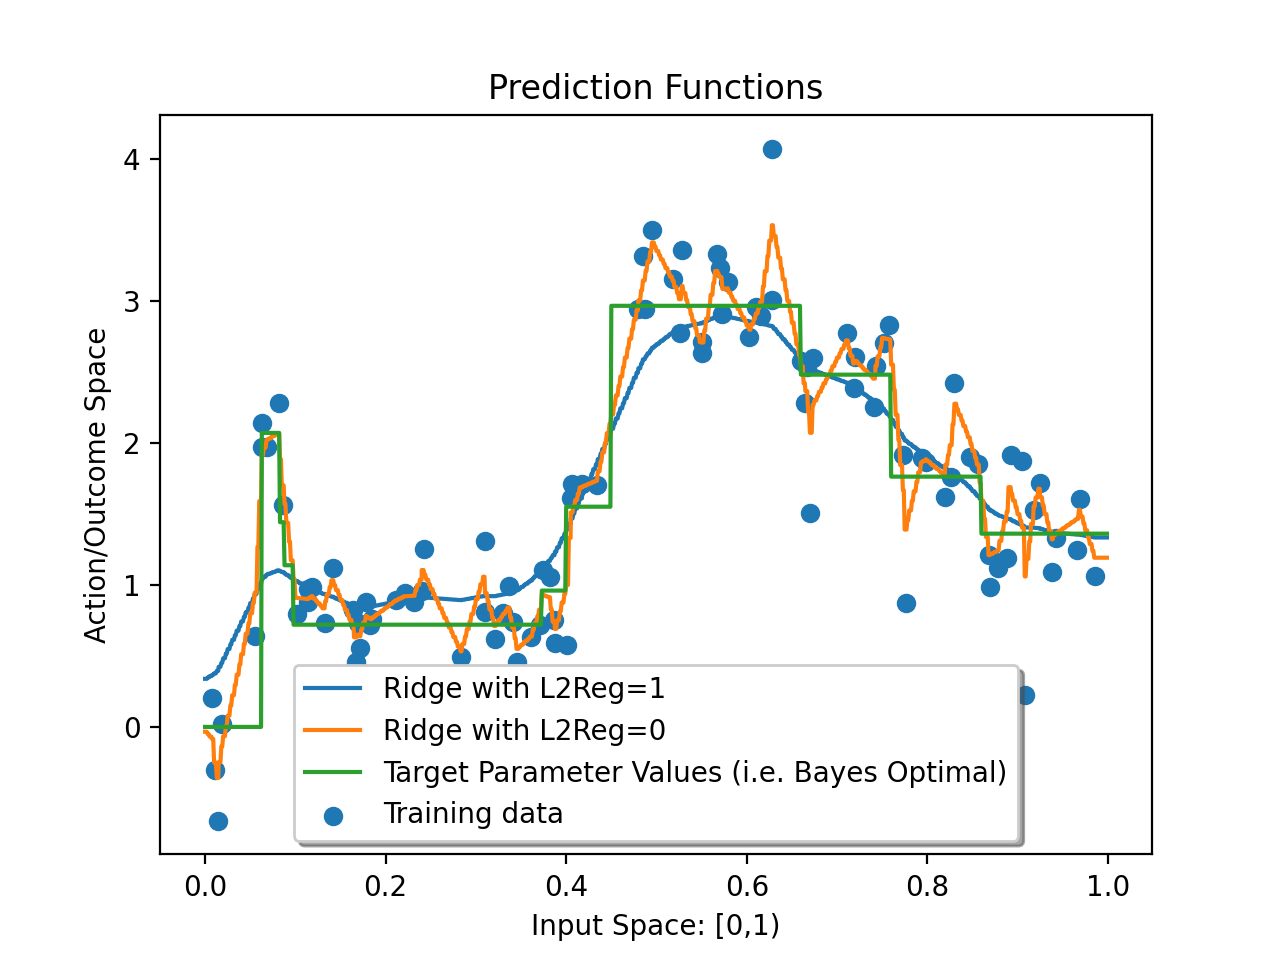
\includegraphics[scale=.7]{Ridge Regression plot.png}
    \caption{Plot of Ridge Regression Function}
    \label{fig:ridge plot}
\end{figure}
Epoch  0 : Ave objective= 1.6239215396574016  Ave training loss:  0.829453172961588
Epoch  50 : Ave objective= 0.3279290433014191  Ave training loss:  0.24172708726984105
Epoch  100 : Ave objective= 0.3162914498004661  Ave training loss:  0.21217722541565676
Epoch  150 : Ave objective= 0.31393109789649476  Ave training loss:  0.2035621043730588
Epoch  200 : Ave objective= 0.3125125713798402  Ave training loss:  0.2001356855415311
Epoch  250 : Ave objective= 0.3119400564708615  Ave training loss:  0.19965745539619076
Epoch  300 : Ave objective= 0.31207381347038765  Ave training loss:  0.19790617941810598
Epoch  350 : Ave objective= 0.31071724617823365  Ave training loss:  0.19849725926934042
Epoch  400 : Ave objective= 0.30909123840416197  Ave training loss:  0.19769513064580496
Epoch  450 : Ave objective= 0.3095956300923911  Ave training loss:  0.19947123786346668
Epoch  500 : Ave objective= 0.3106691495858917  Ave training loss:  0.19746671340931904
Epoch  550 : Ave objective= 0.3097702703398206  Ave training loss:  0.1975530030565645
Epoch  600 : Ave objective= 0.3096404461483278  Ave training loss:  0.19757342715060294
Epoch  650 : Ave objective= 0.3083718030493469  Ave training loss:  0.19798154668862517
Epoch  700 : Ave objective= 0.3061819997787804  Ave training loss:  0.20096498299523102
Epoch  750 : Ave objective= 0.30749345254109606  Ave training loss:  0.20011306539220786
Epoch  800 : Ave objective= 0.308886136728931  Ave training loss:  0.19780391185875232
Epoch  850 : Ave objective= 0.3087756131500073  Ave training loss:  0.1979265611692196
Epoch  900 : Ave objective= 0.3079008111420143  Ave training loss:  0.19828758687030695
Epoch  950 : Ave objective= 0.30714000150784715  Ave training loss:  0.19918632705454822
Epoch  1000 : Ave objective= 0.3066139625516689  Ave training loss:  0.1983538577667799
Epoch  1050 : Ave objective= 0.30747453428905724  Ave training loss:  0.19820704824051763
Epoch  1100 : Ave objective= 0.307717086685998  Ave training loss:  0.19846361621089495
Epoch  1150 : Ave objective= 0.3071694530616267  Ave training loss:  0.19842395292093531
Epoch  1200 : Ave objective= 0.30674000718540045  Ave training loss:  0.19898645299672726
Epoch  1250 : Ave objective= 0.30699547023638646  Ave training loss:  0.19895396194344603
Epoch  1300 : Ave objective= 0.30642748711226797  Ave training loss:  0.1985901886833973
Epoch  1350 : Ave objective= 0.30615191656287044  Ave training loss:  0.199005159544057
Epoch  1400 : Ave objective= 0.3060371837844445  Ave training loss:  0.19891405876500912
Epoch  1450 : Ave objective= 0.3062969093476848  Ave training loss:  0.19899046363269882
Epoch  1500 : Ave objective= 0.305438561622688  Ave training loss:  0.19894348007805548
Epoch  1550 : Ave objective= 0.30504945078923296  Ave training loss:  0.19973854031118024
Epoch  1600 : Ave objective= 0.3056182509567906  Ave training loss:  0.1993384607112306
Epoch  1650 : Ave objective= 0.30516021965519713  Ave training loss:  0.1997367416480982
Epoch  1700 : Ave objective= 0.30612457725427844  Ave training loss:  0.1994450493029651
Epoch  1750 : Ave objective= 0.30534247389005786  Ave training loss:  0.19963722970707437
Epoch  1800 : Ave objective= 0.30323881967916166  Ave training loss:  0.19947349139237075
Epoch  1850 : Ave objective= 0.30511616661964014  Ave training loss:  0.19967194537598545
Epoch  1900 : Ave objective= 0.3051455341157816  Ave training loss:  0.19947225697730386

\setcounter{saveenum}{\value{enumi}}
\end{enumerate}

\section{Multilayer Perceptron}

Let's now turn to a multilayer perceptron (MLP)
with a single hidden layer and a square loss. We'll implement the
computation graph illustrated below:
\begin{center}
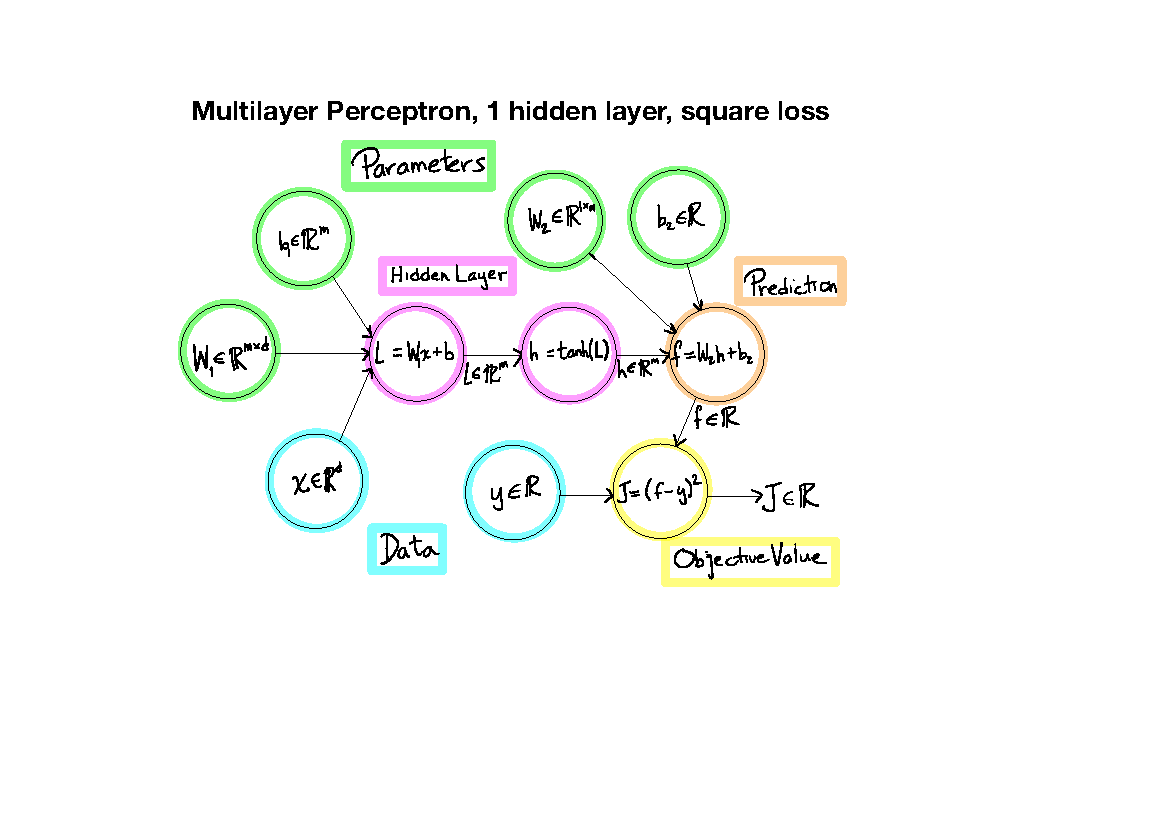
\includegraphics{MLP-computation-graph.pdf}
\par\end{center}

The crucial new piece here is the nonlinear \textbf{hidden layer},
which is what makes the multilayer perceptron a significantly larger
hypothesis space than linear prediction functions.

\subsection{The standard non-linear layer}

The multilayer perceptron consists of a sequence of ``layers'' implementing
the following non-linear function
\[
h(x)=\sigma\left(Wx+b\right),
\]
where $x\in\reals^{d}$, $W\in\reals^{m\times d},$ and $b\in\reals^{m}$,
and where $m$ is often referred to as the number of\textbf{ hidden
units }or\textbf{ hidden nodes}. $\sigma$ is some non-linear function,
typically $\tanh$ or ReLU, applied element-wise to the argument of
$\sigma$. Referring to the computation graph illustration above,
we will implement this nonlinear layer with two nodes, one implementing
the affine transform $L=W_{1}x+b_{1}$, and the other implementing
the nonlinear function $h=\tanh(L)$. In this problem, we'll work
out how to implement the backward method for each of these nodes.

\nyuparagraph{The Affine Transformation}

In a general neural network, there may be quite a lot of computation
between any given affine transformation $Wx+b$ and the final objective
function value $J$. We will capture all of that in a function $f:\reals^{m}\to\reals$,
for which $J=f(Wx+b)$. Our goal is to find the partial derivative
of $J$ with respect to each element of $W$, namely $\partial J/\partial W_{ij}$,
as well as the partials $\partial J/\partial b_{i}$, for each element
of $b$. For convenience, let $y=Wx+b$, so we can write $J=f(y)$.
Suppose we have already computed the partial derivatives of $J$ with
respect to the entries of $y=\left(y_{1},\ldots,y_{m}\right)^{T}$,
namely $\frac{\partial J}{\partial y_{i}}$ for $i=1,\ldots,m$. Then
by the chain rule, we have
\[
\frac{\partial J}{\partial W_{ij}}=\sum_{r=1}^{m}\frac{\partial J}{\partial y_{r}}\frac{\partial y_{r}}{\partial W_{ij}}.
\]

\begin{enumerate}
\setcounter{enumi}{\value{saveenum}}
\item Show that $\frac{\partial J}{\partial W_{ij}}=\frac{\partial J}{\partial y_{i}}x_{j}$,
where $x=\left(x_{1},\ldots,x_{d}\right)^{T}$. {[}Hint: Although
not necessary, you might find it helpful to use the notation $\delta_{ij}=\begin{cases}
1 & i=j\\
0 & \text{else}
\end{cases}$. So, for examples, $\partial_{x_{j}}\left(\sum_{i=1}^{n}x_{i}^{2}\right)=2x_{i}\delta_{ij}=2x_{j}$.{]}

\subitem 

To answer this question we must calculate $\frac{\partial y_r}{\partial W_{ij}}$:

If we nudge the entry $i,j$ of the weight matrix $W$ we have changes corresponding as following:

$$
    \frac{\partial y_r}{\partial W_{ij}} \rightarrow \begin{cases}
    x_j & \ if \ r=j \\
    0 & \ if \ otherwise
    \end{cases}
$$
This is clear to see by the definition of matrix - vector multiplication. If we have Ax = b then $b_i = \langle A_i,x\rangle$ where $A_i$ is the $i^{th}$ row of the matrix A. If we hold all of the other indices of the W matrix constant, that is to say $W_{r,k}$ is constant where $r,j \neq i,j$, then when we take the partial derivative of $y$ with respect to $W_{i,j}$, those constants go to 0. Therefore, when we evaluate the derivative of our dot product $\langle A_i,x\rangle$, we get a summation of 0's with one term that is non zero, $x_j$:
$$
   \frac{\partial y_r}{\partial W_{ij}} \rightarrow \langle W_i, x\rangle = \sum_{r=1}^d \delta_{ij} \times x_r = x_j \ where \ \delta_{ij} \rightarrow \begin{cases}
    x_j & \ if \ r=j \\
    0 & \ if \ otherwise
    \end{cases}
$$

Therefore, what we have is:

$$
\frac{\partial J}{\partial W_{ij}}=\frac{\partial J}{\partial y_{i}}x_{j}
$$



\item Now let's vectorize this. Let's write $\frac{\partial J}{\partial y}\in\reals^{m\times1}$
for the column vector whose $i$th entry is $\frac{\partial J}{\partial y_{i}}$.
Let's also define the matrix $\frac{\partial J}{\partial W}\in\reals^{m\times d}$,
whose $ij$'th entry is $\frac{\partial J}{\partial W_{ij}}$. Generally
speaking, we'll always take $\frac{\partial J}{\partial A}$ to be
an array of the same size (``shape'' in numpy) as $A$. Give a vectorized
expression for $\frac{\partial J}{\partial W}$ in terms of the column
vectors $\frac{\partial J}{\partial y}$ and $x$. {[}Hint: Outer
product.{]}\\

\subitem

We want a matrix $\frac{\partial J}{\partial W}\in\reals^{m\times d}$ whose $ij$'th takes the form $\frac{\partial J}{\partial W_{ij}}$. If we're given $\frac{\partial J}{\partial y}\in\reals^{m\times1}$ then what we need is a vector in $\reals^{1 \times d}$ to take the outer product with to create our $\frac{\partial J}{\partial W}$ matrix.

We know from the last problem that 
$$
\frac{\partial J}{\partial W_{ij}}=\frac{\partial J}{\partial y_{i}}x_{j}
$$
Its easy to see that if we take the outer product of the vector $\frac{\partial J}{\partial y} \in \reals^{m \times 1}$and the vector $x \in \reals^{1\times d}$ then we'll have a matrix 
$$
 \frac{\partial J}{\partial y} \otimes x = \frac{\partial J}{\partial y}x^T \rightarrow \left(\frac{\partial J}{\partial y}\otimes x\right)_{i,j} = \left(\frac{\partial J}{\partial y}\right)_i x_j \ \textit{therefore} \  \frac{\partial J}{\partial y} \otimes x =  \frac{\partial J}{\partial W} 
$$

\item In the usual way, define $\frac{\partial J}{\partial x}\in\reals^{d}$,
whose $i$'th entry is $\frac{\partial J}{\partial x_{i}}$. Show
that 
\[
\frac{\partial J}{\partial x}=W^{T}\left(\frac{\partial J}{\partial y}\right)
\]
{[}Note, if $x$ is just data, technically we won't need this derivative.
However, in a multilayer perceptron, $x$ may actually be the output
of a previous hidden layer, in which case we will need to propagate
the derivative through $x$ as well.{]} \\

\subitem

Using the chain rule, we know that Then the partial of J with respect to an $x_j$ is: 

$$\frac{\partial J}{\partial x_j} = \sum_{i=1}^m \frac{\partial J}{\partial y_i} \frac{\partial y_i}{\partial x_j}$$ 

If we consider the change of $x_j$ as it corresponds to the output of $y_i$:
$$
    \frac{\partial y_i}{\partial x_j} = W_{ij}
$$
Therefore, if were summing over m, we have:
$$
    \frac{\partial J}{\partial x_j} = \sum_{i=1}^m \frac{\partial J}{\partial y_i} W_{ij} = \langle \frac{\partial J}{\partial y}, W_j \rangle = \langle W_j, \frac{\partial J}{\partial y},\rangle = W_j^T \frac{\partial J}{\partial y}
$$
Where we can see that the partial derivative of J with respect to $x_j$ is a linear combination of the entries of W scaled by the partial derivatives of $J$ with respect to $y_i$. If we compute all of the partial derivatives at once, we arrive at our desired equivalency:
$$
    \frac{\partial J}{\partial x} = W^T \frac{\partial J}{\partial y}
$$



\item Show that $\frac{\partial J}{\partial b}=\frac{\partial J}{\partial y}$,
where $\frac{\partial J}{\partial b}$ is defined in the usual way.\\

The vector b, is just the linear bias term, a vector with values are equal to a single variable. Hence, its derivative will always be 1:
$$
    \frac{\partial y_i}{\partial b} = 1
$$
Using the chain rule:
$$
    \frac{\partial J}{\partial b}= \frac{\partial J}{\partial y_i} \frac{y_i}{b}=\sum_{i=1}^m \frac{\partial J}{\partial y_{i}} \times 1 = \frac{\partial J}{\partial y}
$$
\setcounter{saveenum}{\value{enumi}}
\end{enumerate}


\nyuparagraph{Element-wise Transformers}

Our nonlinear activation function nodes take an array (e.g. a vector,
matrix, higher-order tensor, etc), and apply the same nonlinear transformation
$\sigma:\reals\to\reals$ to every element of the array. Let's abuse
notation a bit, as is usually done in this context, and write $\sigma(A)$
for the array that results from applying $\sigma(\cdot)$ to each
element of $A$. If $\sigma$ is differentiable at $x\in\reals$,
then we'll write $\sigma'(x)$ for the derivative of $\sigma$ at
$x$, with $\sigma'(A)$ defined analogously to $\sigma(A)$.

Suppose the objective function value $J$ is written as $J=f(\sigma(A))$,
for some function $f:S\mapsto\reals$, where $S$ is an array of the
same dimensions as $\sigma(A)$ and $A$. As before, we want to find
the array $\frac{\partial J}{\partial A}$ for any $A$. Suppose for
some $A$ we have already computed the array $\frac{\partial J}{\partial S}=\frac{\partial f(S)}{\partial S}$
for $S=\sigma(A)$. At this point, we'll want to use the chain rule
to figure out $\frac{\partial J}{\partial A}$. However, because we're
dealing with arrays of arbitrary shapes, it can be tricky to write
down the chain rule. Appropriately, we'll use a tricky convention:
We'll assume all entries of an array $A$ are indexed by a single
variable. So, for example, to sum over all entries of an array $A$,
we'll just write $\sum_{i}A_{i}$. 
\begin{enumerate}
\setcounter{enumi}{\value{saveenum}}
\item Show that $\frac{\partial J}{\partial A}=\frac{\partial J}{\partial S}\odot\sigma'(A)$,
where we're using $\odot$ to represent the \textbf{Hadamard product}.
If $A$ and $B$ are arrays of the same shape, then their Hadamard
product $A\odot B$ is an array with the same shape as $A$ and $B$,
and for which $\left(A\odot B\right)_{i}=A_{i}B_{i}$. That is, it's
just the array formed by multiplying corresponding elements of $A$
and $B$. Conveniently, in \texttt{numpy} if \texttt{A} and \texttt{B}
are arrays of the same shape, then \texttt{A{*}B} is their Hadamard
product.

\subitem

We know that the derivative of the non linear transformation $\sigma(\cdot)$ is $\sigma'(\cdot)$, therefore, applying the derivative to A we have $\frac{\partial \sigma}{\partial A} = \sigma'(A)$.
We want to compute $\frac{\partial J}{\partial A}$, using the chain rule we know this is equal to:
$$
\frac{\partial J}{\partial A} = \frac{\partial J}{\partial S} \frac{\partial S}{\partial A} 
$$
% We're given in the problem statement that
% $$
% \frac{\partial J}{\partial S} = \frac{\partial f(S)}{\partial S}
% $$
Lets observe what happens when we change a single entry, i, from our array A.
$$
    \frac{\partial S}{\partial A_i} = \frac{\partial \sigma(A)}{\partial A_i} = \sigma'(A_i)
$$

Where $S=\sigma(A)$ and $f(S)$ maps $S$ to $\reals$ for every element of the array. Since what we have is a an arbitrary mapping of every element of S through $f(S)$, and the mapping of $\reals$ to $\reals$ from $\sigma'(A)$ each element of S is a multiplication of two reals, dependent on the inputs of $A_i$ and the output of $\sigma(A_i)$:
$$
    \frac{\partial J}{\partial A_i}=
    \frac{\partial J}{\partial S_i}\frac{\partial S}{\partial A_i} 
    = \frac{\partial J}{\partial S_i}\frac{\partial \sigma(A)}{\partial A_i} 
    = \frac{\partial J}{\partial S_i}\sigma'(A)
    \rightarrow \frac{\partial J}{\partial A}=\frac{\partial J}{\partial S} \odot\sigma'(A)
$$
where $\odot$ is the element wise Hadamard product.

\setcounter{saveenum}{\value{enumi}}
\end{enumerate}

\subsection{MLP Implementation}
\begin{enumerate}
\setcounter{enumi}{\value{saveenum}}

\newpage

\begin{figure}
    \centering
    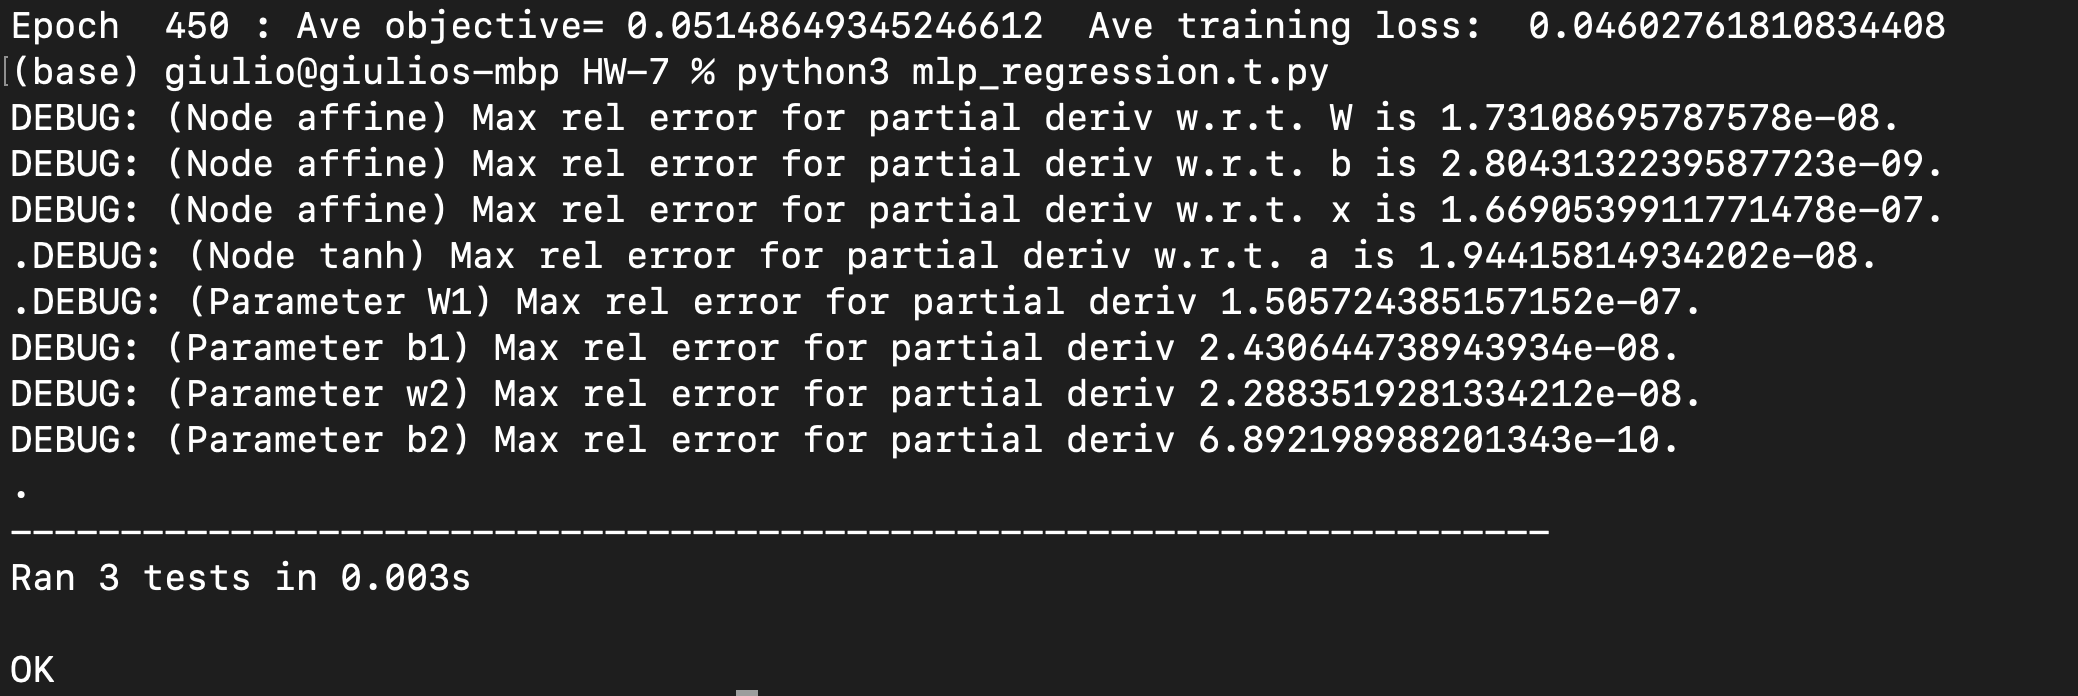
\includegraphics[scale=.4]{MLP Test Output.png}
    \caption{MLP Test Outputs}
    \label{fig:MLP Test}
\end{figure}

\item Complete the class \texttt{AffineNode} in \texttt{nodes.py}. Be sure
to propagate the gradient with respect to $x$ as well, since when
we stack these layers, $x$ will itself be the output of another node
that depends on our optimization parameters. If your code is correct, you should be able to pass test\_AffineNode in \texttt{mlp\_regression.t.py}. Please attach a screenshot that shows the test results for this question.

\subitem

\begin{minted}{Python}
class AffineNode(object):
    """Node implementing affine transformation (W,x,b)-->Wx+b, where W is a matrix,
    and x and b are vectors
        Parameters:
        W: node for which W.out is a numpy array of shape (m,d)
        x: node for which x.out is a numpy array of shape (d)
        b: node for which b.out is a numpy array of shape (m) (i.e. vector of length m)
    """
    def __init__(self, W, x, b,node_name):
        """ 
        Parameters:
        W: node for which w.out is a numpy matrix
        x: node for which a.out is a numpy array
        b: node for which b.out is a numpy array of the same shape as a
        node_name: node's name (a string)
        """
        self.node_name = node_name
        self.out = None
        self.d_out = None
        self.W = W
        self.b = b
        self.x = x

    def forward(self):
        self.out = np.matmul(self.W.out, self.x.out) + self.b.out
        self.d_out = np.zeros(self.out.shape)
        return self.out

    def backward(self):
        #Use derivatives we calculated in homework
        self.W.d_out = np.ma.outer(self.d_out, self.x.out)
        self.b.d_out = self.d_out
        self.x.d_out = np.matmul(self.W.out.T, self.d_out)
        return self.d_out

    def get_predecessors(self):
        # Your code
        return [self.W,self.b,self.x]
\end{minted}

\item Complete the class \texttt{TanhNode} in \texttt{nodes.py}. As you'll
recall, $\frac{d}{dx}\tanh(x)=1-\tanh^{2}x$. Note that in the forward
pass, we'll already have computed $\tanh$ of the input and stored
it in self.out. So make sure to use \texttt{self.out} and not recalculate
it in the backward pass. If your code is correct, you should be able to pass test\_TanhNode in \texttt{mlp\_regression.t.py}. Please attach a screenshot that shows the test results for this question.
\subitem
\begin{minted}{Python}
class TanhNode(object):
    """Node tanh(a), where tanh is applied elementwise to the array a
        Parameters:
        a: node for which a.out is a numpy array
    """
    def __init__(self, a,node_name):
        """ 
        Parameters:
        a: node for which a.out is a numpy array
        node_name: node's name (a string)
        """
        self.node_name = node_name
        self.out = None
        self.d_out = None
        self.a = a

    def forward(self):
        self.out = np.tanh(self.a.out)
        self.d_out = np.zeros(self.out.shape)
        return self.out

    def backward(self):
        #Use derivatives we calculated in homework
        self.a.d_out = self.d_out * (1 - (self.out**2))
        return self.d_out

    def get_predecessors(self):
        return [self.a]
\end{minted}

\item Implement an MLP by completing the skeleton code in \texttt{mlp\_regression.py}
and making use of the nodes above. Your code should pass the tests
provided in \texttt{mlp\_regression.t.py}. Note that to break the symmetry
of the problem, we initialize our weights to small random values,
rather than all zeros, as we often do for convex optimization problems.
Run the MLP for the two settings given in the \texttt{main()} function
and report the average \textbf{training} error. Note that with an
MLP, we can take the original scalar as input, in the hopes that it
will learn nonlinear features on its own, using the hidden layers.
In practice, it is quite challenging to get such a neural network
to fit as well as one where we provide features.
\subitem

\begin{figure}[h!]
    \centering
    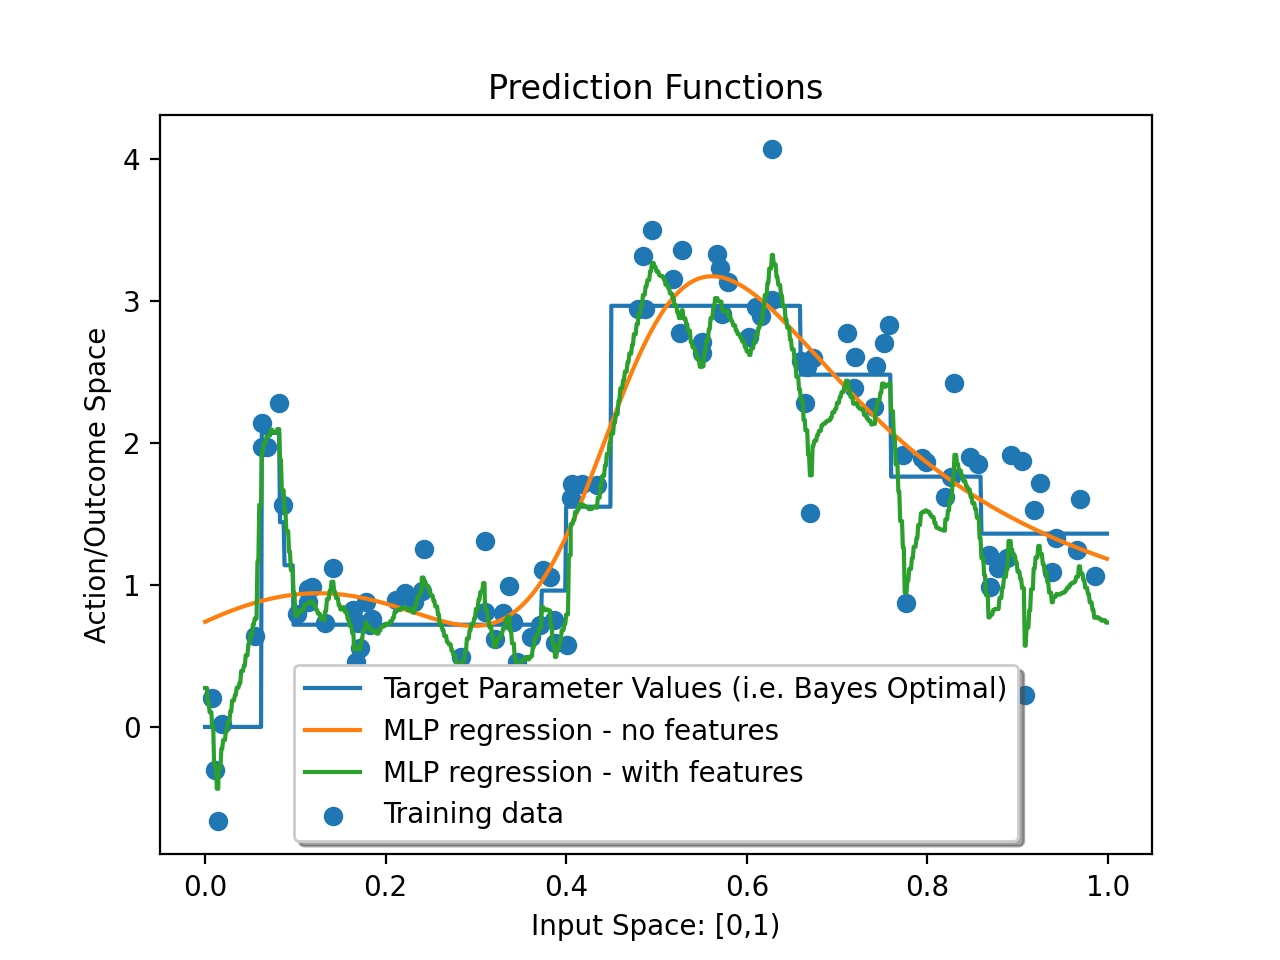
\includegraphics[scale=.7]{MLP Plot output.png}
    \caption{MLP Plot output}
    \label{fig:MLP Plot output}
\end{figure}

\begin{minted}{Python}
class MLPRegression(BaseEstimator, RegressorMixin):
    """ MLP regression with computation graph """
    def __init__(self, num_hidden_units=10, step_size=.005, init_param_scale=0.01, max_num_epochs=5000):
        #Given Params
        self.num_hidden_units = num_hidden_units
        self.init_param_scale = init_param_scale
        self.max_num_epochs = max_num_epochs
        self.step_size = step_size
        #Value Nodes
        self.y = nodes.ValueNode(node_name="y")  # to hold a vector input
        self.x = nodes.ValueNode(node_name="x")  # to hold a vector input
        self.W1 = nodes.ValueNode(node_name="W1")
        self.w2 = nodes.ValueNode(node_name="w2")
        self.b1 = nodes.ValueNode(node_name="b1")
        self.b2 = nodes.ValueNode(node_name="b2")
        #Package Arguments
        self.inputs = [self.x]
        self.outcomes = [self.y]
        self.parameters = [self.W1, self.b1, self.w2, self.b2]
        #Transformation Nodes
        self.matrixAffineNode = nodes.AffineNode(
            W=self.W1, x=self.x, b=self.b1, node_name="Matrix-Vector Affine Node")
        self.tanh = nodes.TanhNode(
            a=self.matrixAffineNode, node_name="TanH node")
        self.prediction = nodes.VectorScalarAffineNode(
            x=self.tanh, b=self.b2, w=self.w2, node_name="Vector
    Scalar Affine Prediction Node")
        self.objective = nodes.SquaredL2DistanceNode(
            a=self.prediction, b=self.y, node_name="Squared Distance Node")
        self.graph = graph.ComputationGraphFunction(self.inputs, self.outcomes,
                                                    self.parameters, self.prediction,
                                                    self.objective)
\end{minted}
Epoch  0 : Ave objective= 3.1384886539883388  Ave training loss:  2.723785243910098
Epoch  50 : Ave objective= 0.9452874177705872  Ave training loss:  0.943461455298143
Epoch  100 : Ave objective= 0.9445033731029092  Ave training loss:  0.942652506502907
Epoch  150 : Ave objective= 0.9367476670890391  Ave training loss:  0.9346090461873809
Epoch  200 : Ave objective= 0.8844483557361549  Ave training loss:  0.8810580089341782
Epoch  250 : Ave objective= 0.7915298648457691  Ave training loss:  0.7875920118136019
Epoch  300 : Ave objective= 0.7675597340207823  Ave training loss:  0.7633388588307334
Epoch  350 : Ave objective= 0.7602930361825055  Ave training loss:  0.7564261106066077
Epoch  400 : Ave objective= 0.7524547326529253  Ave training loss:  0.7484077188972953
Epoch  450 : Ave objective= 0.7428788443128451  Ave training loss:  0.738966672345131
Epoch  500 : Ave objective= 0.7321920184466244  Ave training loss:  0.7288235006540531
Epoch  550 : Ave objective= 0.7222214365888472  Ave training loss:  0.7187396934421737
Epoch  600 : Ave objective= 0.7130055930160536  Ave training loss:  0.7092100547107983
Epoch  650 : Ave objective= 0.7044883875478416  Ave training loss:  0.7007717624558434
Epoch  700 : Ave objective= 0.6969450741027985  Ave training loss:  0.6935702346255589
Epoch  750 : Ave objective= 0.6910156523283387  Ave training loss:  0.6875683109990217
Epoch  800 : Ave objective= 0.6862222329256947  Ave training loss:  0.6824991754483698
Epoch  850 : Ave objective= 0.6819994828642706  Ave training loss:  0.6781000976663271
Epoch  900 : Ave objective= 0.6773895074147217  Ave training loss:  0.6740627739647225
Epoch  950 : Ave objective= 0.6736227015552761  Ave training loss:  0.669864085725015
Epoch  1000 : Ave objective= 0.6693218243530432  Ave training loss:  0.6653432766719775
Epoch  1050 : Ave objective= 0.6643837895234525  Ave training loss:  0.6601950629134805
Epoch  1100 : Ave objective= 0.6585088963124851  Ave training loss:  0.6539338279490771
Epoch  1150 : Ave objective= 0.6510972305836367  Ave training loss:  0.6462104106767659
Epoch  1200 : Ave objective= 0.6415259617630464  Ave training loss:  0.6364378999285787
Epoch  1250 : Ave objective= 0.6295993066336498  Ave training loss:  0.6242604999266641
Epoch  1300 : Ave objective= 0.6142219153217402  Ave training loss:  0.6082239068761517
Epoch  1350 : Ave objective= 0.5954813684673169  Ave training loss:  0.5888388672455861
Epoch  1400 : Ave objective= 0.5709948524358075  Ave training loss:  0.5659841940822471
Epoch  1450 : Ave objective= 0.5430969069160582  Ave training loss:  0.5404888850053465
Epoch  1500 : Ave objective= 0.5146237289009121  Ave training loss:  0.5082343319474094
Epoch  1550 : Ave objective= 0.48356823492449197  Ave training loss:  0.47586773954280814
Epoch  1600 : Ave objective= 0.4514673318252107  Ave training loss:  0.44358943167442194
Epoch  1650 : Ave objective= 0.42216074491521666  Ave training loss:  0.4138969070261208
Epoch  1700 : Ave objective= 0.3959897535492102  Ave training loss:  0.3882628148595082
Epoch  1750 : Ave objective= 0.37463870229920154  Ave training loss:  0.36757513611321946
Epoch  1800 : Ave objective= 0.3594697433958645  Ave training loss:  0.3520927159473004
Epoch  1850 : Ave objective= 0.34629722997211343  Ave training loss:  0.34081126371663695
Epoch  1900 : Ave objective= 0.33292407430679505  Ave training loss:  0.334826289682421
Epoch  1950 : Ave objective= 0.33221653382092337  Ave training loss:  0.3246279741340167
Epoch  2000 : Ave objective= 0.3254469869100473  Ave training loss:  0.3195559080130552
Epoch  2050 : Ave objective= 0.3191475404122815  Ave training loss:  0.31602858351100305
Epoch  2100 : Ave objective= 0.3194399126729073  Ave training loss:  0.310987799563054
Epoch  2150 : Ave objective= 0.31347039708863256  Ave training loss:  0.3095644700210537
Epoch  2200 : Ave objective= 0.30925097045693034  Ave training loss:  0.30628300955673343
Epoch  2250 : Ave objective= 0.30815239160309493  Ave training loss:  0.302177619523987
Epoch  2300 : Ave objective= 0.305460336189331  Ave training loss:  0.29903566851895924
Epoch  2350 : Ave objective= 0.3026997974708049  Ave training loss:  0.29636267413752004
Epoch  2400 : Ave objective= 0.3004278784672875  Ave training loss:  0.29484270071893703
Epoch  2450 : Ave objective= 0.2986209840718123  Ave training loss:  0.29220179992469186
Epoch  2500 : Ave objective= 0.29228630014181634  Ave training loss:  0.29300318803571096
Epoch  2550 : Ave objective= 0.2950618790412984  Ave training loss:  0.28805881036612
Epoch  2600 : Ave objective= 0.2923601903618309  Ave training loss:  0.2866935017033392
Epoch  2650 : Ave objective= 0.29148179187751955  Ave training loss:  0.28448913111610524
Epoch  2700 : Ave objective= 0.28896976044790185  Ave training loss:  0.2829393560287766
Epoch  2750 : Ave objective= 0.2868191289049734  Ave training loss:  0.28137306934023487
Epoch  2800 : Ave objective= 0.28531300657157144  Ave training loss:  0.2798083898582309
Epoch  2850 : Ave objective= 0.2842080841525052  Ave training loss:  0.2781184660054683
Epoch  2900 : Ave objective= 0.28271008763298594  Ave training loss:  0.27661781946323705
Epoch  2950 : Ave objective= 0.2806229154132455  Ave training loss:  0.27540973147311154
Epoch  3000 : Ave objective= 0.2796565925441325  Ave training loss:  0.2738203206425151
Epoch  3050 : Ave objective= 0.2764865169964034  Ave training loss:  0.27447982849389996
Epoch  3100 : Ave objective= 0.2763603740746643  Ave training loss:  0.2715763865913923
Epoch  3150 : Ave objective= 0.27558867438514956  Ave training loss:  0.2703350929006941
Epoch  3200 : Ave objective= 0.27444147940519065  Ave training loss:  0.2686737759054997
Epoch  3250 : Ave objective= 0.27203739375033714  Ave training loss:  0.26824221780073015
Epoch  3300 : Ave objective= 0.27179551223861614  Ave training loss:  0.2663827986195835
Epoch  3350 : Ave objective= 0.26964341016686966  Ave training loss:  0.26626356176210825
Epoch  3400 : Ave objective= 0.26804093348640645  Ave training loss:  0.2655768577899346
Epoch  3450 : Ave objective= 0.26632823817318807  Ave training loss:  0.2642029002460602
Epoch  3500 : Ave objective= 0.2673348358188661  Ave training loss:  0.26265675013281986
Epoch  3550 : Ave objective= 0.2647839016616244  Ave training loss:  0.2622159813318914
Epoch  3600 : Ave objective= 0.26462533335380395  Ave training loss:  0.26204829869432755
Epoch  3650 : Ave objective= 0.2639994700194897  Ave training loss:  0.25906637418812495
Epoch  3700 : Ave objective= 0.2617166615490344  Ave training loss:  0.2596774688183659
Epoch  3750 : Ave objective= 0.26165028350887537  Ave training loss:  0.2574431609637332
Epoch  3800 : Ave objective= 0.26174575538285344  Ave training loss:  0.2563592205344483
Epoch  3850 : Ave objective= 0.26050615894939877  Ave training loss:  0.25603940761988975
Epoch  3900 : Ave objective= 0.25938168132136885  Ave training loss:  0.2546501240398735
Epoch  3950 : Ave objective= 0.2587562436576191  Ave training loss:  0.2542149655292055
Epoch  4000 : Ave objective= 0.2573923586445567  Ave training loss:  0.2534187670327716
Epoch  4050 : Ave objective= 0.2575037498261381  Ave training loss:  0.25222824572726765
Epoch  4100 : Ave objective= 0.2567433957573593  Ave training loss:  0.2514705797058361
Epoch  4150 : Ave objective= 0.254539201860611  Ave training loss:  0.25081065052643925
Epoch  4200 : Ave objective= 0.2551022001931922  Ave training loss:  0.2500129556752864
Epoch  4250 : Ave objective= 0.2524591307616317  Ave training loss:  0.2511660755294462
Epoch  4300 : Ave objective= 0.253606426978595  Ave training loss:  0.2485668066428239
Epoch  4350 : Ave objective= 0.25224274642086864  Ave training loss:  0.24804124753794388
Epoch  4400 : Ave objective= 0.25171003798259906  Ave training loss:  0.24718285629754916
Epoch  4450 : Ave objective= 0.2518032563510767  Ave training loss:  0.24668291744528095
Epoch  4500 : Ave objective= 0.2509992469334581  Ave training loss:  0.24596185427796008
Epoch  4550 : Ave objective= 0.25049238776736305  Ave training loss:  0.2452602339866061
Epoch  4600 : Ave objective= 0.24667098437191168  Ave training loss:  0.24469438801640678
Epoch  4650 : Ave objective= 0.24868314822435666  Ave training loss:  0.24402846433041894
Epoch  4700 : Ave objective= 0.24835918306678365  Ave training loss:  0.24374840714503526
Epoch  4750 : Ave objective= 0.24813844789514078  Ave training loss:  0.24286703419961467
Epoch  4800 : Ave objective= 0.2467084452633521  Ave training loss:  0.2436449712832135
Epoch  4850 : Ave objective= 0.2460279568646779  Ave training loss:  0.24217766666977902
Epoch  4900 : Ave objective= 0.2465078880032288  Ave training loss:  0.24132104095532025
Epoch  4950 : Ave objective= 0.24568467743447064  Ave training loss:  0.24067333063364513
Epoch  0 : Ave objective= 3.2800713177228773  Ave training loss:  2.853580140086361
Epoch  50 : Ave objective= 0.14933163110436884  Ave training loss:  0.14641707217182806
Epoch  100 : Ave objective= 0.11796958226228409  Ave training loss:  0.10897419879235355
Epoch  150 : Ave objective= 0.10134139201573841  Ave training loss:  0.09053530456233325
Epoch  200 : Ave objective= 0.08369303494526008  Ave training loss:  0.08057937150782428
Epoch  250 : Ave objective= 0.07773935817925802  Ave training loss:  0.06512939388553708
Epoch  300 : Ave objective= 0.06421651532868872  Ave training loss:  0.10111298800424694
Epoch  350 : Ave objective= 0.06279796009585302  Ave training loss:  0.05203375968856143
Epoch  400 : Ave objective= 0.0527607128276177  Ave training loss:  0.04706368772606726
Epoch  450 : Ave objective= 0.049430156701997664  Ave training loss:  0.04412280461792682
\setcounter{saveenum}{\value{enumi}}
\end{enumerate}

\subsection{Multiclass classification with an MLP (Optional)}
We consider a generic classification problem with $K$ classes over inputsn 
$x$ of dimension $d$. Using a MLP we will compute a K-dimensional vector $z$ representing scores, 
$$
z = W_2 \tanh (W_1 x + b_1) + b_2,
$$
with $W_1 \in \reals^{m\times d}$, $b_1 \in \reals^m$, $W_2 \in \reals^{K \times m}$ and $b_1 \in \reals^K$.
Our model assumes that $x$ belongs to class $k$ with probability $$ e^{z_k}/\sum_{k=1}^K e^{z_k},$$
which corresponds to applying a Softmax to the scores. Given this probabilistic model we can train the model by minimizing the negative log-likelihood.
\begin{enumerate}
\setcounter{enumi}{\value{saveenum}}
\item Implement a Softmax node. We provided skeleton code for class SoftmaxNode in \texttt{nodes.py}. If your code is correct, you should be able to pass test\_SoftmaxNode in \texttt{multiclass.t.py}. Please attach a screenshot that shows the test results for this question.

\begin{figure}
    \centering
    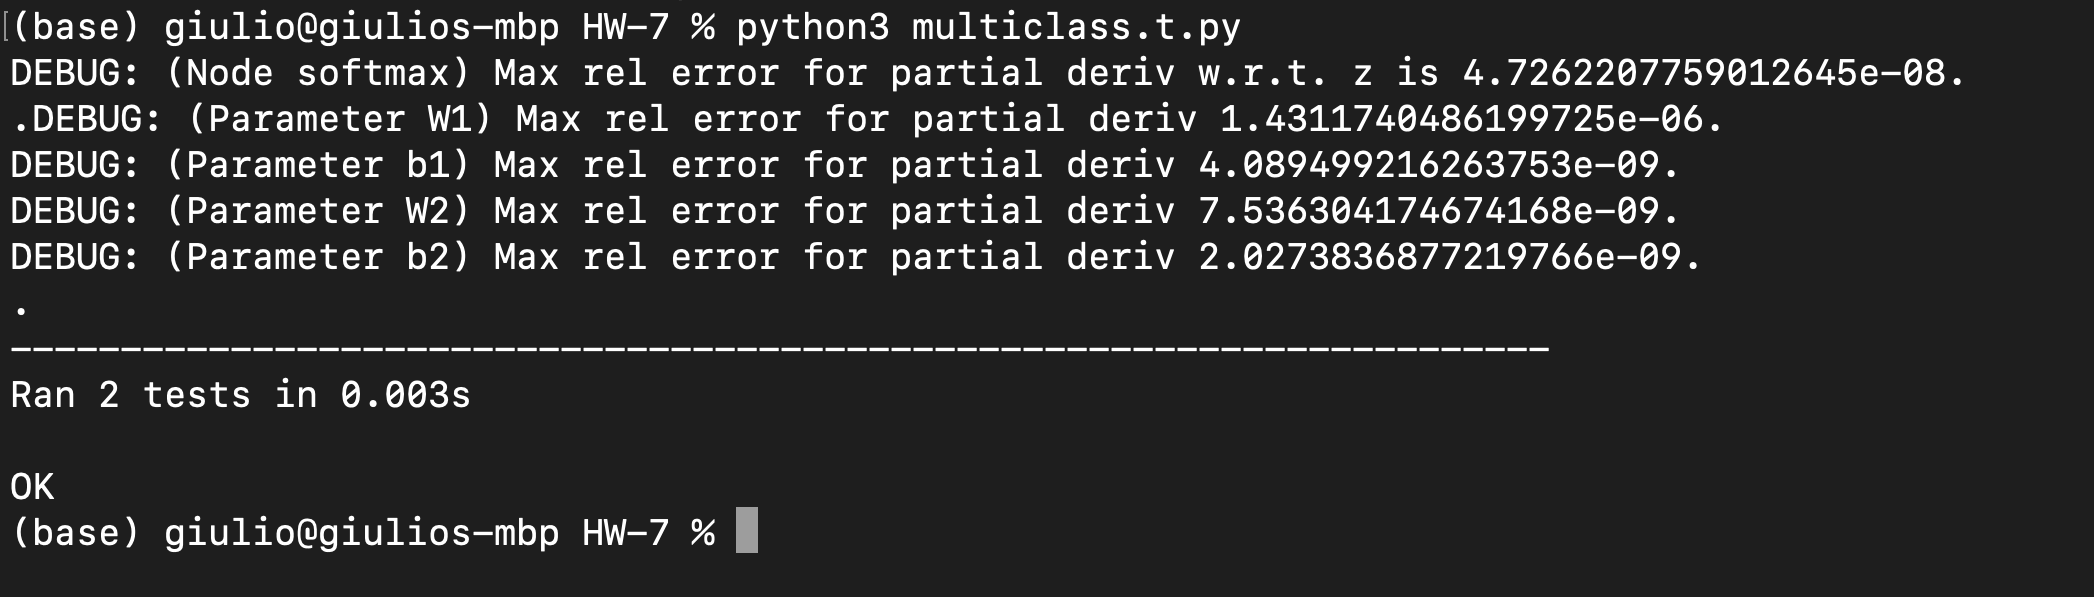
\includegraphics[scale=.4]{Multiclass test.png}
    \caption{Multiclass test}
    \label{fig:Multiclass test}
\end{figure}

\subitem
\begin{minted}{Python}
class SoftmaxNode(object):
    """ Softmax node
        Parameters:
        z: node for which z.out is a numpy array
    """
    def __init__(self,z,node_name) -> None:
        self.node_name = node_name
        self.z = z
        self.d_out = None
        self.out = None 

    def forward(self):
        self.out = np.exp(self.z.out) /  np.sum(np.exp(self.z.out))
        self.d_out = np.zeros(self.out.shape)
        return self.out

    def backward(self):
        jacobian = -np.outer(self.out, self.out)
        np.fill_diagonal(jacobian, self.out*(1-self.out))
        self.z.d_out = self.d_out @ jacobian
        return self.d_out

    def get_predecessors(self):
        return [self.z]
\end{minted}

\item Implement a negative log-likelihood loss node for multiclass
classification. We provided skeleton code for class NLLNode in \texttt{nodes.py}. The test code for this question is combined with the test code for the next question.

\subitem
\begin{minted}{Python}
class NLLNode(object):
    """ Node computing NLL loss between 2 arrays.
        Parameters:
        y_hat: a node that contains all predictions
        y_true: a node that contains all labels
    """
    def __init__(self,y_hat,y_true,node_name) -> None:
        self.out = None
        self.d_out = None
        self.y_hat = y_hat
        self.y_true = y_true
        self.node_name = node_name
        self.temp = None
        
    def forward(self):    
        self.temp = self.y_hat.out[self.y_true.out]
        self.out = -np.log(self.temp)
        self.d_out = np.zeros(self.out.shape)
        return self.out

    def backward(self):
        self.temp2 = np.zeros(self.y_hat.out.shape)
        self.temp2[self.y_true.out] = -1*(self.temp**-1)
        self.y_hat.d_out = self.d_out * self.temp2
        return self.d_out

    def get_predecessors(self):
        return [self.y_hat,self.y_true]
\end{minted}
\item Implement a MLP for multiclass classification by completing the skeleton code in \texttt{multiclass.py}. Your code should pass the tests in test\_multiclass provided in multiclass.t.py. Please attach a screenshot that shows the test results for this question.

\subitem
\begin{minted}{Python}
class MulticlassClassifier(BaseEstimator, RegressorMixin):
    """ Multiclass prediction """
    def __init__(self, num_hidden_units=10, step_size=.005, init_param_scale=0.01, 
                                                max_num_epochs=1000, num_class=3):
        self.num_hidden_units = num_hidden_units
        self.init_param_scale = init_param_scale
        self.max_num_epochs = max_num_epochs
        self.step_size = step_size
        self.num_class = num_class

        # Build computation graph
        # TODO: add your code here
        self.z = nodes.ValueNode(node_name='z')
        self.x = nodes.ValueNode(node_name='x')
        self.y = nodes.ValueNode(node_name='y')
        self.W1 = nodes.ValueNode(node_name='W1')
        self.W2 = nodes.ValueNode(node_name='W2')
        self.b1 = nodes.ValueNode(node_name='b1')
        self.b2 = nodes.ValueNode(node_name='b2')

        # Package inputs / parameters into lists
        self.inputs = [self.x, self.z]
        self.outcomes = [self.y]
        self.parameters = [self.W1, self.b1, self.W2, self.b2]

        # First We Start With Affine Transformation W_1x+b_1
        self.MatVecAffine1 = nodes.AffineNode(
            W=self.W1, x=self.x, b=self.b1, node_name="Mat-Vec Affine Node 1")
        # Which feeds into a tahn layer
        self.tahnNode = nodes.TanhNode(
            a=self.MatVecAffine1, node_name="TahnNode")
        # Tahn node feeds into another Affine transformation -> W_2tahn + b_1
        self.MatVecAffine2 = nodes.AffineNode(
            W=self.W2, x=self.tahnNode, b=self.b2, node_name="Mat-Vec Affine Node 2")
        # Which becomes z, and fed into our softmax, creates prediction
        self.prediction = nodes.SoftmaxNode(
            z=self.MatVecAffine2, node_name="SoftMax Prediction Node")
        # Finally evaluated againts objective of NLL
        self.objective = nodes.NLLNode(
            y_hat=self.prediction, y_true=self.y, node_name="NLL Objective Node")

        # Build Computation Graph
        self.graph = graph.ComputationGraphFunction(
            inputs=self.inputs, outcomes=self.outcomes, parameters=self.parameters, 
            prediction=self.prediction, objective=self.objective)
\end{minted}


Epoch  0  Ave training loss:  0.10767753468425854
Epoch  50  Ave training loss:  0.003740272949801889
Epoch  100  Ave training loss:  0.0019509875089186053
Epoch  150  Ave training loss:  0.0013189220100329906
Epoch  200  Ave training loss:  0.0009947600104512845
Epoch  250  Ave training loss:  0.0007975221227264001
Epoch  300  Ave training loss:  0.0006649220947379011
Epoch  350  Ave training loss:  0.0005697138957458585
Epoch  400  Ave training loss:  0.0004980771960410213
Epoch  450  Ave training loss:  0.00044225221211177576
Epoch  500  Ave training loss:  0.0003975450315101266
Epoch  550  Ave training loss:  0.0003609495175393885
Epoch  600  Ave training loss:  0.0003304520224436157
Epoch  650  Ave training loss:  0.0003046529432352649
Epoch  700  Ave training loss:  0.0002825495526238341
Epoch  750  Ave training loss:  0.00026340479431621313
Epoch  800  Ave training loss:  0.00024666486030361454
Epoch  850  Ave training loss:  0.0002319056839595022
Epoch  900  Ave training loss:  0.0002187970217752761
Epoch  950  Ave training loss:  0.00020707801611844284
Test set accuracy = 1.000

\setcounter{saveenum}{\value{enumi}}
\end{enumerate}

\end{document}

